\documentclass[conference]{IEEEtran}
\IEEEoverridecommandlockouts
% The preceding line is only needed to identify funding in the first footnote. If that is unneeded, please comment it out.
\usepackage{cite}
\usepackage{amsmath,amssymb,amsfonts}
%\usepackage{algorithm}
\usepackage{algorithmic}
\usepackage{graphicx}
\usepackage{textcomp}
\usepackage{xcolor}
\usepackage[lined,algonl,boxed]{algorithm2e}
\usepackage{xspace}

\def\BibTeX{{\rm B\kern-.05em{\sc i\kern-.025em b}\kern-.08em
    T\kern-.1667em\lower.7ex\hbox{E}\kern-.125emX}}
\begin{document}




\title{ELEN4020: Data Intensive Computing\\ Lab 2\\
{\footnotesize School of Electrical \& Information Engineering, University of the
Witwatersrand, Private Bag 3, 2050, Johannesburg, South Africa}
%\thanks{Identify applicable funding agency here. If none, delete this.}
}


\author{

\IEEEauthorblockN{Elias Sepuru 1427726}
\and
\IEEEauthorblockN{Boikanyo Radiokana 1386807}
\and
\IEEEauthorblockN{Lloyd Patsika 1041888}

}

\maketitle

%\begin{abstract}
%This document is a model and instructions for \LaTeX.
%This and the IEEEtran.cls file define the components of your paper [title, text, heads, etc.]. *CRITICAL: Do Not Use Symbols, Special Characters, Footnotes, 
%or Math in Paper Title or Abstract.
%\end{abstract}

%\begin{IEEEkeywords}
%component, formatting, style, styling, insert
%\end{IEEEkeywords}

\section{INTRODUCTION}
This document provides a brief explanation of the algorithms used to transpose 2D large matrices using shared memory programming libraries, Pthread and OpenMP. The parallel programming libraries are compiled in the Linux environment using C. The performance of the different algorithms with and without the parallel programming libraries are compared and analysed. The sizes of the matrices that are transposed are: 128, 1024, 2048 and 4096 respectively. The number of threads for both Pthreads and OpenMP are set to 8 for all the algorithms.

\section{Naive Transposition}

\subsection{Basic}
The algorithm involves iterating the whole 2D matrix using two nested for loops for the row and column respectively. The element at index [i,j] is swapped with the element at index [j,i] using a temporary variable. The pseudo code \ref{basic} below shows the algorithm used in the \texttt{NaiveTransposeBasic(twoD)} function.

%\linesnumbered
\begin{algorithm}

%\centring

\SetKwData{temp}{temp}
%\SetKwData{C}{C}
%\SetKwData{tempVector}{tempVector}
%\SetKwFunction{Union}{Union}
%\SetKwFunction{FindCompress}{FindCompress}
\SetKwInOut{Input}{input}
%\SetKwInOut{Output}{output}


\caption{\texttt{NaiveTransposeBasic(twoD)}}\Input{2D matrix of size $n\times n$}
%\Output{A resultant C 2D matrix}
%%\BlankLine\emph{special treatment of the first line}\;
\For{$i\gets0$ \KwTo $n-1$}{
%\emph{special treatment of the first element of line $i$}\;
     \For{$j\gets0$ \KwTo $i$}{
%\nllabel{forins}
         \temp$\leftarrow${$A[i,j]$}\;
         {$A[i,j]$}$\leftarrow${$A[j,i]$}\;
         {$A[j,i]$}$\leftarrow$\temp\;
}

}
\label{basic}
\end{algorithm}

\subsection{OpenMP}
The number of threads set for Naive threading is set at 8. The varaibles i and j, indices of rows and  columns are defined inside the pragma statement which sets them to be private by default. The directives used for the parallelism of the two nested for loops are:\\

\begin{itemize}
    \item \texttt{\textbf{\#pragma omp parallel}}
    \item \texttt{\textbf{\#pragama omp for nowait}}
\end{itemize}

%The use of the \texttt{nowait} clause allows threads that have completed the tasks to carry on with the next code in the parallel region.
%The second direct


The use of the \texttt{nowait} clause allows threads that have completed the tasks to carry on with the next code in the parallel region. The second directive distributes the iterations of the for loop to the threads for execution.  The algorithm \ref{2} below shows the pseudo code implemented in the function.

\begin{algorithm}

%\centring

\SetKwData{temp}{temp}
%\SetKwData{C}{C}
%\SetKwData{tempVector}{tempVector}
%\SetKwFunction{Union}{Union}
%\SetKwFunction{FindCompress}{FindCompress}
\SetKwInOut{Input}{input}
%\SetKwInOut{Output}{output}


\caption{\texttt{NaiveTransposeBasic(twoD)}}\Input{2D matrix of size $n\times n$}
%\Output{A resultant C 2D matrix}
%%\BlankLine\emph{special treatment of the first line}\;
\texttt{\#pragma omp parallel}{\\
\For{$i\gets0$ \KwTo $n-1$}{
%\emph{special treatment of the first element of line $i$}\;
     \texttt{\#pragma omp for nowait}\\
     \For{$j\gets0$ \KwTo $i$}{
%\nllabel{forins}
         \temp$\leftarrow${$A[i,j]$}\;
         {$A[i,j]$}$\leftarrow${$A[j,i]$}\;
         {$A[j,i]$}$\leftarrow$\temp\;
}
}
}
\label{2}
\end{algorithm}

\section{Diagonal Transposition}
\subsection{Basic}
The algorithm involves iterating the 2D matrix along the main diagonal of the matrix. At each diagonal, the matrix is transposed by swapping the elements in the corresponding row with the elements in the corresponding column. The element at index [i,j] is swapped with the element at index [j,i]. 

\begin{algorithm}

%\centring

\SetKwData{temp}{temp}
%\SetKwData{C}{C}
%\SetKwData{tempVector}{tempVector}
%\SetKwFunction{Union}{Union}
%\SetKwFunction{FindCompress}{FindCompress}
\SetKwInOut{Input}{input}
%\SetKwInOut{Output}{output}


\caption{\texttt{DiagonalTransposeBasic(twoD)}}\Input{2D matrix of size $n\times n$}
%\Output{A resultant C 2D matrix}
%%\BlankLine\emph{special treatment of the first line}\;
\For{$i\gets0$ \KwTo $n-1$}{
%\emph{special treatment of the first element of line $i$}\;
     \For{$j\gets{i+1}$ \KwTo $n-1$}{
%\nllabel{forins}
         \temp$\leftarrow${$A[i,j]$}\;
         {$A[i,j]$}$\leftarrow${$A[j,i]$}\;
         {$A[j,i]$}$\leftarrow$\temp\;
}

}
\label{basic}
\end{algorithm}

\subsection{OpenMP}
The same methodology used in the Naive-OpenMP threading is used because the structure of the code is the same, the only difference is the way the matrix is accessed which can be seen in the pseudo code above. The two directives used are:

\begin{itemize}
    \item \texttt{\textbf{\#pragma omp parallel}}
    \item \texttt{\textbf{\#pragama omp for nowait}}
\end{itemize}

The pseudo code below shows the use of OpenMP threads in the diagonal threading algorithm.
\begin{algorithm}

%\centring

\SetKwData{temp}{temp}
\SetKwInOut{Input}{input}



\caption{\texttt{DiagonalTransposeBasic(twoD)}}\Input{2D matrix of size $n\times n$}
\texttt{\#pragma omp parallel}\\
\For{$i\gets0$ \KwTo $n-1$}{
     \texttt{\#pragma omp for nowait}\\
     \For{$j\gets{i+1}$ \KwTo $n-1$}{
         \temp$\leftarrow${$A[i,j]$}\;
         {$A[i,j]$}$\leftarrow${$A[j,i]$}\;
         {$A[j,i]$}$\leftarrow$\temp\;
}

}
\label{basic}
\end{algorithm}


\subsection{Pthreads}
The Diagonal Transpose using Pthreads algorithm is built on top of the basic diagonal transpose method. This means that the swapping along the diagonals is the same, however the code is now executed using 8 parallel threads. Each thread is initially assigned to a diagonal, and this assignment is dependent on the size of the matrix. Since the sizes for this lab's matrices are all greater than 8, each thread does get assigned an initial diagonal to perform a diagonal transpose on. The need for the threads to be re-assigned new diagonals as well as make sure the threads are always in sync and do not edit an already transposed diagonal resulted in: a \texttt{While-Loop} that continues  until a \texttt{break} due to the next possible thread being the second last diagonal, \texttt{N-1}, as well as \texttt{Pthread$\_$Mutex$\_$Lock} and \texttt{Pthread$\_$Mutex$\_$Unlock} being used to keep the threads in sync, as well as assign a new diagonal to a thread. The pseudo code can be seen in Algorithm \ref{diag}.


\begin{algorithm}[h!]

%\centring

\SetKwData{temp}{temp}
%\SetKwData{C}{C}
%\SetKwData{tempVector}{tempVector}
%\SetKwFunction{Union}{Union}
%\SetKwFunction{FindCompress}{FindCompress}
\SetKwInOut{Input}{input}
%\SetKwInOut{Output}{output}


\caption{\texttt{DiagonalTransposePThread(*agms)}}\Input{A \texttt{Struct} with 2D matrix of size $n\times n$, Diagonal, Matrix Size}
%\Output{A resultant C 2D matrix}
%%\BlankLine\emph{special treatment of the first line}\;
\While{true}
{
\For{$i\gets0$ \KwTo $n-1$}{
%\emph{special treatment of the first element of line $i$}\;
     \For{$j\gets{i+1}$ \KwTo $n-1$}{
%\nllabel{forins}
         \temp$\leftarrow${$A[i,j]$}\;
         {$A[i,j]$}$\leftarrow${$A[j,i]$}\;
         {$A[j,i]$}$\leftarrow$\temp\;
}

}

\texttt{Pthread$\_$Mutex$\_$Lock}


\If{nextDiagonal $<$ SIZE-1}{

currentDiagonal = nextDiagonal\\
++nextDiagonal}
\Else{currentDiagonal = SIZE-1}

\texttt{Pthread$\_$Mutex$\_$Unlock}\\
\If{currentDiagonal == SIZE-1} {BREAK}
}
\label{diag}
\end{algorithm}

\section{Blocked Transposition}
\subsection{Basic}
Block Transposition of a matrix involves splitting the matrix in to equal sub-matrices, each sub-matrix is then transposed. After the transposition of each sub-matrix, the sub-matrices are 'seen' as elements of the original/bigger matrix. The original matrix is then transposed with elements being the sub-matrices. Algorithm \ref{block} represent the algorithm that was used to transpose each sub-matrix. 

\begin{algorithm}[h!]


\SetKwData{temp}{temp}
\SetKwData{otherCol}{otherCol}
\SetKwData{otherRow}{otherRow}
\SetKwData{A}{A}
\SetKwFunction{swap}{swap}
%\SetKwFunction{FindCompress}{FindCompress}
\SetKwInOut{Input}{input}
%\SetKwInOut{Output}{output}
\caption{\texttt{blockElementTranspose(A)}}\Input{A 2D matrix "A" of size $n\times n$}

\otherCol$\leftarrow$0
\\
\otherRow$\leftarrow$0

%\Output{A resultant C 2D matrix}
%%\BlankLine\emph{special treatment of the first line}\;
\For{$i\gets0$ \KwTo $n-1$}{
\For{$j\gets0$ \KwTo $n-1$}{
%\emph{special treatment of the first element of line $i$}\;
     \For{$k\gets{0}$ \KwTo $BLOCK\_SIZE$}{
%\nllabel{forins}
          \For{$l\gets{0}$ \KwTo $l < k$}{
         
            \If{$i != j$}{
                   \otherRow$\leftarrow(i + l)$
                   \otherCol$\leftarrow(j + k)$   
               }
              \Else{
                    \otherRow$\leftarrow(l+j)$
                    \otherCol$\leftarrow(k+i)$   
                  }
          
            
           \swap($A[k+i][l+j]$, $A[\otherRow][\otherCol]$)
            }
}

}
}

\label{block}
\end{algorithm}


To transpose the blocks the function \texttt{blockTranspose(A)} was used. Algorithm \ref{blockB} presents the pseudocode for the  \texttt{blockTranspose(A)} function.


\begin{algorithm}[h!]

%\centring

\SetKwData{temp}{temp}
%\SetKwData{C}{C}
%\SetKwData{tempVector}{tempVector}
\SetKwFunction{blockSwap}{blockSwap}
%\SetKwFunction{FindCompress}{FindCompress}
\SetKwInOut{Input}{input}
%\SetKwInOut{Output}{output}


\caption{\texttt{blockTranspose(A)}}\Input{2D matrix "A" of size $n\times n$}
%\Output{A resultant C 2D matrix}
%%\BlankLine\emph{special treatment of the first line}\;
\For{$i\gets0$ \KwTo $n-1$}{
%\emph{special treatment of the first element of line $i$}\;
     \For{$j\gets{0}$ \KwTo $j < i$}{
%\nllabel{forins}
         \blockSwap($i,j,A$)
}

}
\label{blockB}
\end{algorithm}

The \texttt{blockSwap} as seen in Algorithm \ref{blockB} takes in the positions of the blocks where the swaps take place together with a pointer to the matrix.

\subsection{Pthreads}
The Pthreads block threading algorithm was built on top of the basic one. The functions depicted by Algorithm \ref{block} \& \ref{blockB} were altered in way that Pthreads function would work on them. Algorithm \ref{blockT} illustrates how the threads were created for block element transposition. 


\begin{algorithm}[h!]


\SetKwData{temp}{temp}
\SetKwData{otherCol}{otherCol}
\SetKwData{otherRow}{otherRow}
\SetKwData{A}{A}
\SetKwData{break}{break}
\SetKwData{blockThread}{blockThread}
\SetKwFunction{swap}{swap}
%\SetKwFunction{FindCompress}{FindCompress}
\SetKwInOut{Input}{input}
%\SetKwInOut{Output}{output}
\caption{\texttt{PthreadblockElementTranspose(A)}}\Input{A 2D matrix "A" of size $n\times n$}


\While{1}{
\otherCol$\leftarrow$0
\\
\otherRow$\leftarrow$0


%\Output{A resultant C 2D matrix}
%%\BlankLine\emph{special treatment of the first line}\;
\For{$i\gets{\blockThread->row}$ \KwTo $\blockThread->row + BLOCK\_SIZE$}{
\For{$j\gets0$ \KwTo $n-1$}{
%\emph{special treatment of the first element of line $i$}\;
     \For{$k\gets{0}$ \KwTo $BLOCK\_SIZE$}{
%\nllabel{forins}
          \For{$l\gets{0}$ \KwTo $l < k$}{
         
            \If{$i != j$}{
                   \otherRow$\leftarrow(i + l)$
                   \otherCol$\leftarrow(j + k)$   
               }
              \Else{
                    \otherRow$\leftarrow(l+j)$
                    \otherCol$\leftarrow(k+i)$   
                  }
          
            
           \swap($(\blockThread->arr+ (k+i)*SIZE + (l+j)), (\blockThread->arr + (\otherRow)*SIZE + (\otherCol)$)
            }
}

}
}

  
   \If {$NEXT\_ROW\_E >= SIZE - 1$} \break

     $pthread\_mutex\_lock(\&stillBusy)$;
    
     		$\blockThread->row\leftarrow NEXT\_ROW\_E$;
     		$NEXT\_ROW\_E+=BLOCK\_SIZE$

      $pthread\_mutex\_unlock(\&stillBusy)$

}
\label{blockT}
\end{algorithm}

For block transposition a similar approach was followed. Algorithm \ref{2} illustrates.


\begin{algorithm}[h!]

%\centring

\SetKwData{temp}{temp}
%\SetKwData{C}{C}
%\SetKwData{tempVector}{tempVector}
\SetKwFunction{blockSwap}{blockSwap}
%\SetKwFunction{FindCompress}{FindCompress}
\SetKwInOut{Input}{input}
%\SetKwInOut{Output}{output}


\caption{\texttt{blockTranspose(A)}}\Input{2D matrix "A" of size $n\times n$}
%\Output{A resultant C 2D matrix}
%%\BlankLine\emph{special treatment of the first line}\;
\While{1}{
\For{$i\gets{\blockThread->row}$ \KwTo $\blockThread->row+BLOCK\_SIZE$}{
%\emph{special treatment of the first element of line $i$}\;
     \For{$j\gets{0}$ \KwTo $j < i$}{
%\nllabel{forins}
         \blockSwap($i,j,A$)
}

}

 \If {$NEXT\_ROW\_B >= SIZE - 1$} \break

     $pthread\_mutex\_lock(\&stillBusy)$;
    
     		$\blockThread->row\leftarrow NEXT\_ROW\_$;
     		$NEXT\_ROW\_B+=BLOCK\_SIZE$

      $pthread\_mutex\_unlock(\&stillBusy)$

}
\label{2}
\end{algorithm}

\subsection{OpenMP}
The functions  \texttt{blockElementTranspose()} and \texttt{blockTranspose()} are the only functions in the build up of block threading were OpenMP is implemented. The directive used in \texttt{blockElementTranspose()} is a one line parallel construct with the for, private and shared clause.
\begin{itemize}
    \item \texttt{\textbf{#pragma omp parallel for private(otherRow, otherCol) shared(twoD)}}
\end{itemize}

This means that the variables in the private function are not shared between the threads,each thread has its own local copy of the variable. However the twoD array in the shared function is shared between the threads.This means that there is only one instance of the array and multiple threads can access the twoD array at the same time. The directives used in the \texttt{blockTranspose()} function is the same as the Diagonal Transposition for OpenMP since the methodology is the same. Algorithm \ref{blo} shows the pseudo code of the OpenMP Block Threading.

\begin{algorithm}

%\centring

%\SetKwData{BLOCK\_SIZE}{BLOCK\_SIZE}
\SetKwInOut{Input}{input}



\caption{\texttt{blockTransposeBasic(twoD)}}\Input{2D matrix of size $n\times n$}
\texttt{\#pragma omp parallel}\\
\For{$i\gets0$ \KwTo $i+BLOCK\_SIZE$}{
     \texttt{\#pragma omp for nowait}\\
     \For{$j\gets0$ \KwTo $j+BLOCK\_SIZE$}{
         \texttt{blockSwap(i,j,twoD[0])}
}

}
\label{blo}
\end{algorithm}

\subsection{Pthreads}

\section{Timer}
The function \texttt{timer(twoD, type\_transpose)} is a void function that accepts any of the transposing functions as an argument together with a string which is a name of the method used. It uses the \texttt{$gettimeofday()$} function from the sys/time.h preprocessor directive. The timer starts counting just before the transposing function that is passed to the timer function is called. After the transposing function executes the mathematical computations the timer stops counting. The duration of the transposing function is calculated as seen in Algorithm 11 below .The units of the duration is presented in milliseconds.

\begin{algorithm}

%\centring

\SetKwData{duration}{duration}
\SetKwData{start}{start}
%\SetKwData{end}{end}
%\SetKwData{duration}{duration}
%\SetKwData{type_transpose}{type_transpose}
\SetKwFunction{gettimeofday}{gettimeofday}
\SetKwFunction{f}{f}
\SetKwData{dispaly}{display}
\SetKwInOut{Input}{input}
\SetKwFunction{prinf}{prinf}
%\SetKwInOut{Output}{output}


\caption{\texttt{DiagonalTransposeBasic(twoD)}}\Input{2D matrix of size $n\times n$}
\gettimeofday(\& start, $NULL$)\\
\f(twoD)\\
\gettimeofday(\& end, $NULL$)\\
\duration$\leftarrow$((end-start)+1e6*(end-start))*1000\\
display \duration

\label{b}
\end{algorithm}




% The following subsections present the procedures and pseudocode followed in the transposition of 2D matrices using the various methods as well as the different type of shared memory programming libraries.

\section{RESULTS \& ANALYSIS}

The algorithms were run 4 times(see Appendix A) on the same machine at the same conditions to ensure fairness. The average of the 5 readings for each method and size were calculated and recorded in table below.
\begin{table}[h!]
\caption{Perfomance of different sizes with differet methods of threading}
\begin{tabular}{|l|l|l|l|l|l|l|}
\hline
\textbf{\begin{tabular}[c]{@{}l@{}}Matrix sizes \\ nxn\end{tabular}} & Basic & \multicolumn{2}{l|}{Pthreads} & \multicolumn{3}{l|}{OpenMP} \\ \hline
 &  & Diagonal & Blocked & Naive & Diagonal & Blocked \\ \hline
128 & 0.22425 & 2.195 & 11.09 & 1.066 & 0.639 & 0.975 \\ \hline
1024 & 11.311 & 3.123 & 4.321 & 4.201 & 3.329 & 4.849 \\ \hline
2048 & 51.452 & 35.67 & 17.324 & 13.925 & 16.092 & 13.88 \\ \hline
4096 & 244.9605 & 129.8487 & 67.364 & 76.67 & 119.1075 & 57.079 \\ \hline
\end{tabular}
\end{table}
\\
\\From the table above it can be seen the all the basic approaches perform relatively well from sizes 128-2048, however as the sizes increases the threading algorithms prove to be more efficient.   

\section{CONCLUSION}
From the results gathered in the table it can be seen that Block Threading is faster in all of the implementations, with \textttt{OpenMP} taking first place in the implementations. 

\newpage
\onecolumn
\appendix

\begin{figure}[h!]
    \centering
    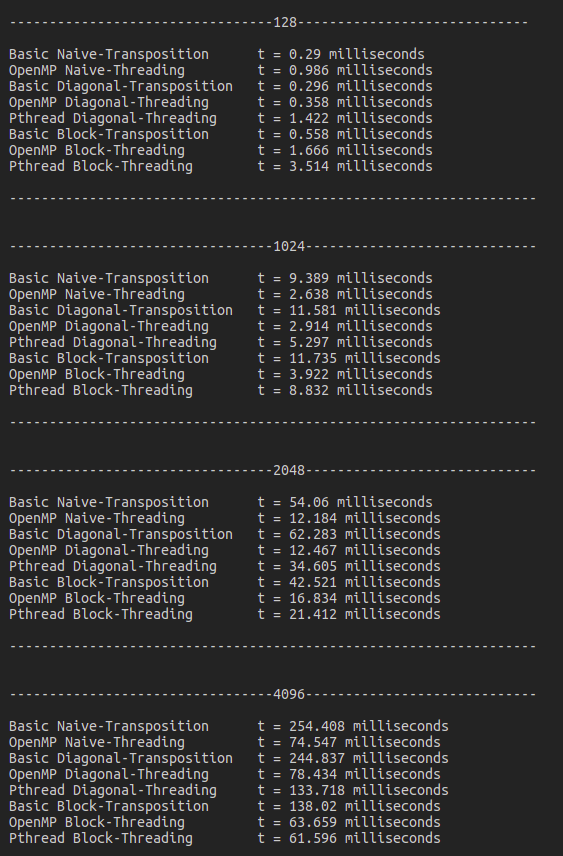
\includegraphics[scale = 0.6]{1a.png}
    \caption{Caption}
    \label{fig:my_label}
\end{figure}

\begin{figure}[h!]
    \centering
    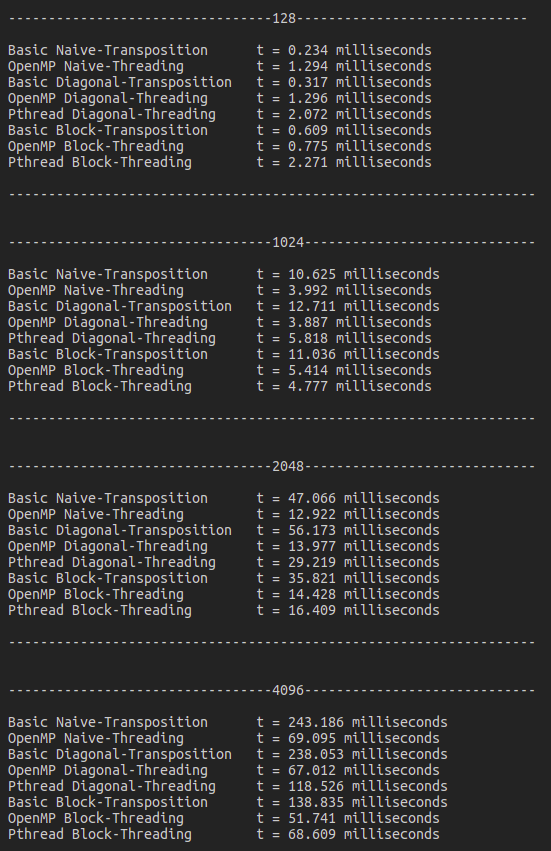
\includegraphics[scale = 0.6]{2a.png}
    \caption{Caption}
    \label{fig:my_label}
\end{figure}

\begin{figure}[h!]
    \centering
    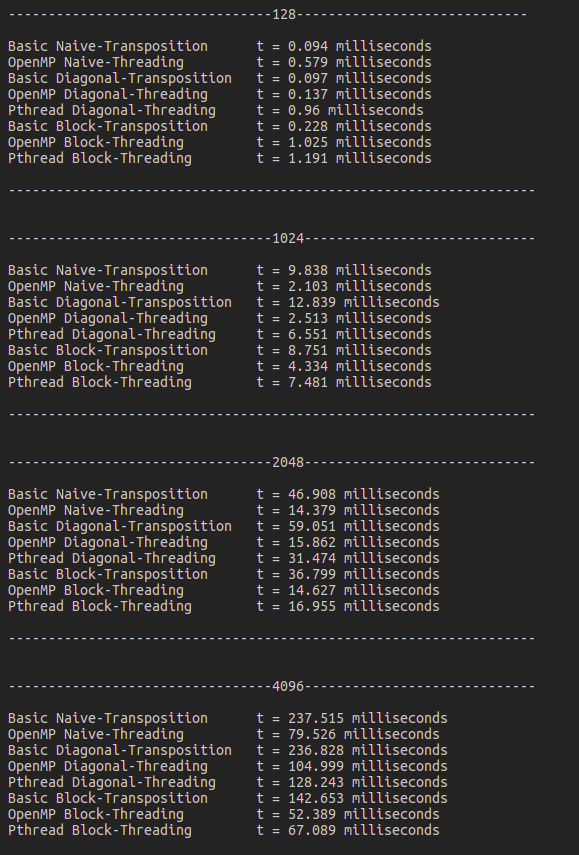
\includegraphics[scale = 0.6]{3b.png}
    \caption{Caption}
    \label{fig:my_label}
\end{figure}

\begin{figure}[h!]
    \centering
    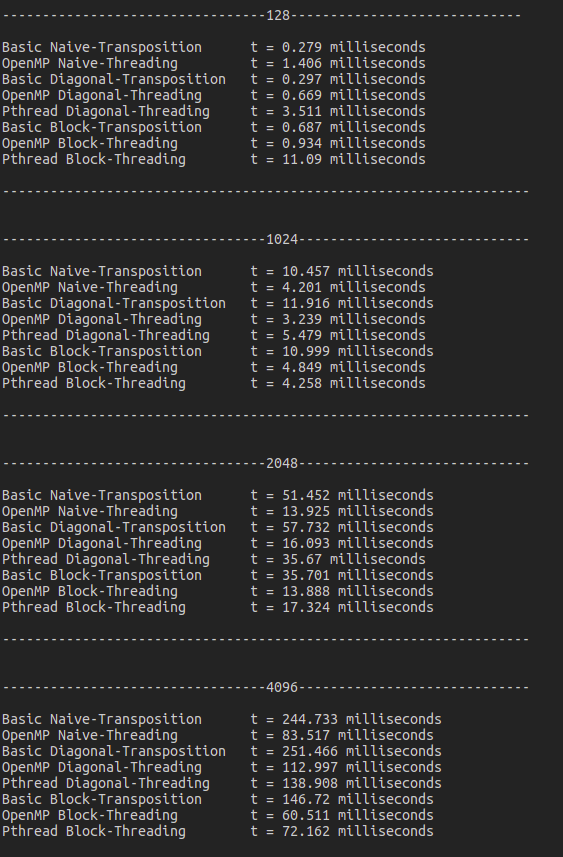
\includegraphics[scale = 0.6]{4b.png}
    \caption{Caption}
    \label{fig:my_label}
\end{figure}



% The implementation of 2D and 3D matrix computations are succesfully executed. The computations are coded in C++. The 2D matrix computation code proved to be reusable in 3D computations, avoiding the DRY principle. The methodology used in the computation of the 3D matrices proved to be using sequential computing as each layer of the final matrix had to wait for another layer to be computed before it could be computed.

%\begin{thebibliography}{00}
%\bibitem{b1} G. Eason, B. Noble, and I. N. Sneddon, ``On certain integrals of Lipschitz-Hankel type involving products of Bessel functions,'' Phil. Trans. Roy. Soc. London, vol. A247, pp. 529--551, April 1955.

%\end{thebibliography}
\vspace{12pt}
%%%%%%%%%%%%%%%%%%%%%%%%%%%%%%%%%%%%%%%%%%%%%%%%%%%%%%%%%%%%%%%%%%%%%%%%%%%%%%%
%



% \subsection{Multiplication of 2D matrices}
% For the multiplication of 2D matrices, the following standard mathematical equation is followed:

% \begin{equation}
% \centering
% 	c_{ij} = \sum_{k} a_{ik}\times b_{kj}
%     \label{eq1}
% \end{equation}

% The function used for the multiplication of the 2D matrices is \texttt{rank2DTensorMult(A,B)} accepting two matrices A and B and returning a resultant matrix C as per equation \ref{eq1}. The following pseudocode represents the internal workings of the \texttt{rank2DTenosrMult(A,B)} function.



% \linesnumbered
% \begin{algorithm}

% \centring

% \SetKwData{tempSum}{tempSum}
% \SetKwData{C}{C}
% \SetKwData{tempVector}{tempVector}
% %\SetKwFunction{Union}{Union}
% %\SetKwFunction{FindCompress}{FindCompress}
% \SetKwInOut{Input}{input}
% \SetKwInOut{Output}{output}


% \caption{\texttt{rank2DTenosrMult(A,B)}: 2D Matrix Multplication}\Input{Two 2D matrices of sizes $n\times n$}
% \Output{A resultant C 2D matrix}
% %%\BlankLine\emph{special treatment of the first line}\;
% \For{$i\gets1$ \KwTo $n$}{
% %\emph{special treatment of the first element of line $i$}\;
%      \For{$j\gets1$ \KwTo $n$}{

% 	\For{$k\gets1$ \KWTo $n$}{
% %\nllabel{forins}
% 	     \tempSum$\leftarrow$ \tempSum + {$A[i,k]\times B[j,k]$}\;
% 	}
% 	\tempVector$\leftarrow$ \tempSum\;
% }

% \C$\leftarrow$ \tempVector\;

% }
% \Return \C
% \label{mult2d}
% \end{algorithm}


% \subsection{Addition of 2D matrices}
% For the addition of 2D matrices, the function \texttt{rank2DTensorAdd(n,A,B)} is used. The function accepts the matrices A and B and also accepts the desired size, n, inputed by the user. The function then returns a resultant C, which is an addition of A and B. Algorithm \ref{add2D} below presents the pseudocode of the function.



% \begin{algorithm}

% \centring

% %\SetKwFunction{Union}{Union}
% %\SetKwFunction{FindCompress}{FindCompress}

% \SetKwData{C}{C}
% \SetKwInOut{Input}{input}
% \SetKwInOut{Output}{output}
% \caption{\texttt{rank2DTenosrAdd(n,A,B)}: 2D Matrix Addition}\Input{size of matrix(n),Two 2D matrices of sizes $n\times n$}
% \Output{A resultant C 2D matrix}
% %%\BlankLine\emph{special treatment of the first line}\;
% \For{$i\gets1$ \KwTo $n$}{
% %\emph{special treatment of the first element of line $i$}\;
%      \For{$j\gets1$ \KwTo $n$}{
	
% %\nllabel{forins}
% 	     {$C[i,j]$}$\leftarrow$ {$A[i,k] + B[j,k]$}\;
	
% }

% }
% \Return \C
% \label{add2D}
% \end{algorithm}


% %%%%%%%%%%%%%%%%%%%%%%%%%%%%%%%%%%%%%%%%%%%%%%%%%%%%%%%%%%%%%
% %%%%%%%%%%%%%%%%%%%%%%%%%%%%%%%%%%%%%%%%%%%%%%%%%%%%%%%%%%%

% \subsection{Multiplication of 3D matrices}
% All the 3D computations adopt the 2D computations discussed in earlier sections. For 3D multiplication, the 3D$n\times n\times n$ matrices are broken down into $n$ 2D matrices of sizes $n\times n$. From there they are passed into the function \texttt{rank2DTensorMult(A,B)} which returns $subC$ of size $n\times n$. The $n\times n$ $subC$ is then used to build an $n\times n\times n$ 3D matrix, C, layer by layer. All of this happens in \texttt{rank3DTensorMult(A,B)} function illustrated by agorithm \ref{mult3D}.


% \linesnumbered

% \begin{algorithm}

% \centring

% \SetKwData{subC}{subC}
% \SetKwData{C}{C}
% \SetKwFunction{rank2DTensorMult}{rank2DTensorMult}
% %\SetKwFunction{Union}{Union}
% %\SetKwFunction{FindCompress}{FindCompress}
% \SetKwInOut{Input}{input}
% \SetKwInOut{Output}{output}


% \caption{\texttt{rank3DTenosrMult(A,B)}: 3D Matrix Multplication}\Input{Two 3D matrices of sizes $n\times n\times n$}
% \Output{A resultant 3D matrix, C}

% \For{$i\gets1$ \KwTo $n$}{

     
% 	     \subC$\leftarrow$ rank2DTensorMult({$A[i],B[i]$})\;
%               \C$[i]\leftarrow$ \subC\;
% 	}

% \Return \C

% \label{mult3D}

% \end{algorithm}


 
% \subsection{Addition of 3D matrices}
% As mentioned earlier 2D computations are used to build up 3D computations. The addition of 3D matrices also adopts the function \texttt{rank2DTensorAdd(n,A,B)} on the break down of 3D matrices into 2D matrices. The function \texttt{rank3DTensorAdd(n,A,B)} is used and algorithm \ref{add3D} illustrates the internal workings of the function.


% \linesnumbered

% \begin{algorithm}[H]

% \centring

% \SetKwData{subC}{subC}
% \SetKwData{C}{C}
% \SetKwFunction{rank2DTensorAdd}{rank2DTensorAdd}
% %\SetKwFunction{Union}{Union}
% %\SetKwFunction{FindCompress}{FindCompress}
% \SetKwInOut{Input}{input}
% \SetKwInOut{Output}{output}


% \caption{\texttt{rank3DTenosrAdd(n,A,B)}: 3D Matrix addition}\Input{Two 3D matrices of sizes $n\times n\times n$}
% \Output{A resultant 3D matrix, C}

% \For{$i\gets1$ \KwTo $n$}{

     
% 	     \subC$\leftarrow$ rank2DTensorAdd({$A[i],B[i]$})\;
%               \C$[i]\leftarrow$ \subC\;
% 	}

% \Return \C

% \label{add3D}

% \end{algorithm}

\end{document}
